\section{Other commonly DWS-Architectures}
\label{sec:otherArchitectures}
After having introduced the reference architecture this chapter aims to show other approaches for building Data-Warehouse-Systems. Main object of consideration is the distributed DWS architecture. This one was invented by Ralph Kimball and can be seen as counterpart to Inmons hub and spoke architecture.\newline
Afterwards the characteristics of different data mart arrangements will be handled. This information will be used later on especially to deal with a flexible data provision.\newline
In the end an outlook upon different options regarding the data persistence in the different layers will be given. This topic will get relevant while talking about the deployment of Data-Warehouse-Systems as collection of micro-services by using the self-contained systems approach.

\subsection{Distributed Data Warehousing Architecture}
After having explained the reference architecture from A. Bauer which implements the hub and spoke idea from Inmon one very common alternative is presented. Ralph Kimball is another pioneer in this area who came up with a distributed data warehousing architecture based upon data marts connected to a bus system. \cite{surveyDWSArchs} Figure \ref{fig:distributedWarehouseArchitecture} visualises this in more detail.
\begin{figure}[htb]
    \centering
    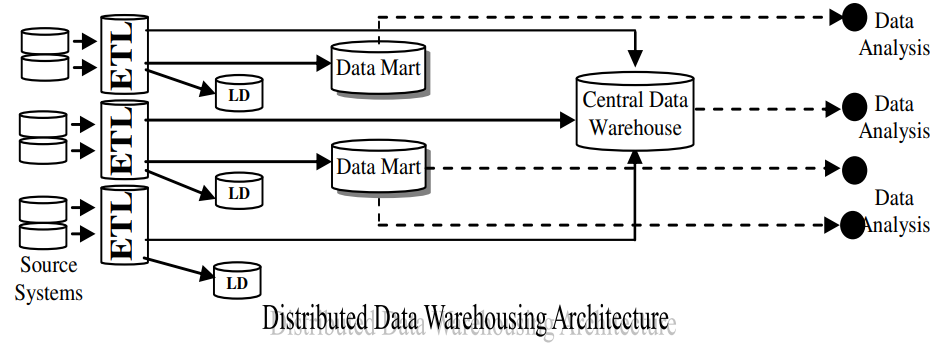
\includegraphics[scale=0.5]{pictures/DistributedDataWarehouseArchitecture.PNG}
    \caption{Distributed Data Warehousing Architecture by Ralph Kimball \cite{surveyDWSArchs}}
    \label{fig:distributedWarehouseArchitecture}
\end{figure}
\\In contrast to Inmon's approach Kimball allows 'Everyone [...] to fabricate their database according to their requirements and department structures. All there independent repositories can be integrated as and when. [...]' \cite{surveyDWSArchs}. Due to that the Central / Core Data Warehouse results from those individual Data Mart and doesn't provide any consistency. This technique is also known as bottom-up approach for developing Data Warehouse Systems. Since the bus system is needed to ensure the interoperability between multiple data marts and the core data warehouse consistent data standards are therefore needed. Due to that the design aspects are quite tough and the complexity is high. \cite{KimbalVSInmon}\newline
As Breslin states 'Kimball's approach is a departure from traditional database development'\cite[p.~19]{KimbalVSInmon} and therefore targets the IT-Professional himself.\newline

\subsection{Architectural Classification according to the Arrangement of Data Marts}
Next to the radical redesign of the hub and spoke architecture by Kimball's distributed data warehousing architecture, some alternatives regarding the organisation of data marts will be shown.\newline
\\
A central Data Warehouse consists of a single central instance with only one data mart which is used for all of the analysis. This can be beneficial when a company-wide overview is needed. On the downside, it is only possible to apply one data model to this data mart. For department-specific analysis this could result in a huge problem. \newline
Instead the use of a distributed Data Warehouse consists of multiple data marts which are department specific. Each of this additional data storage has a separate schema. Due to this the creation of a new one results in more work. Problematic is the company-wide perspective, which will get lost. \newline
A possible combination of the advantages from the two architectures above can be found in a central Data Warehouse with multiple distributed data marts. By applying this concept it is possible to run company-wide analysis upon the central Data Warehouse and using data marts for the individual needs coming from various departments.
\newline
One last aspect which needs to get pointed out is the design aspects of dependent and independent data marts. Therefor lets have a look at dependent ones first. Those are build upon the core data warehouse and might contain additional or aggregated information. Nevertheless the underlying CDW ensures a consistency of the information distributed to the data marts. An independent data mart won't consist of such layer beneath. Due to that the information inside might be duplicated and distinct. An advantage of using an independent architecture is the simplicity of creating those. \cite{scriptRasch} \newline
\\
This section should have shown the various design possibilities of data marts inside a corporate Data Warehouse System. By thinking about a modern adaption of DWS architectures, it is necessary to construct new data marts easily without losing the company-wide point of view and still enable departments to come up with their own requirements for analysis. 

\subsection{Options regarding the persistent Data Handling}
After having introduced various structural options above let us face the topic of data persistence in current Data Warehouse Systems.

\cite{sinz}


After the most commonly used architectures for Data Warehouse Systems have been outlined and the requirements regarding a DWS are pointed out, some newer technologies are introduced. In detail the fundamental ideas of micro-service and event-based architectures as well as Business Process Management will be elaborated. Further on these technologies will align in order to result into the final draft of the presented architecture.